\section{\ac{SCF}\textsuperscript{ARM}: DESIGN AND IMPLEMENTATION}

We have developed the \ac{SCF}\textsuperscript{ARM} specifically for the static analysis of ARMv8-M binaries targeting Cortex-M23, focusing on identifying timing side-channel vulnerabilities. Our approach, centered around symbolic taint-tracking, enables a rapid, cost-effective, and automated assessment of these vulnerabilities. We have implemented an open source  version of \ac{SCF}\textsuperscript{ARM} built upon Angr\footnote{https://angr.io/} and \ac{SCF}\textsuperscript{MSP} \cite{scfmsp}. Specifically, (1) we use Angr for symbolic execution of binaries and conducting Value Set Analysis (\ac{VSA}) to determine potential register values or symbolic memory addresses; (2) we expand the functionality of the \ac{SCF}\textsuperscript{MSP} tool to analyze TrustZone-M targeted binaries and ensure program integrity against a novel DMA-based side-channel attack termed BUSted \cite{busted}. 

Fig. \ref{fig:SCFARM} showcases a high-level workflow diagram detailing the components of the \ac{SCF}\textsuperscript{ARM} tool. The dashed box denotes the core elements implementing our proposed side channel evaluation technique. \ac{SCF}\textsuperscript{ARM} is built on approximately 1110 lines of Python code and integrates various established Python libraries, as detailed in the following.

\begin{figure*}
  \centering
  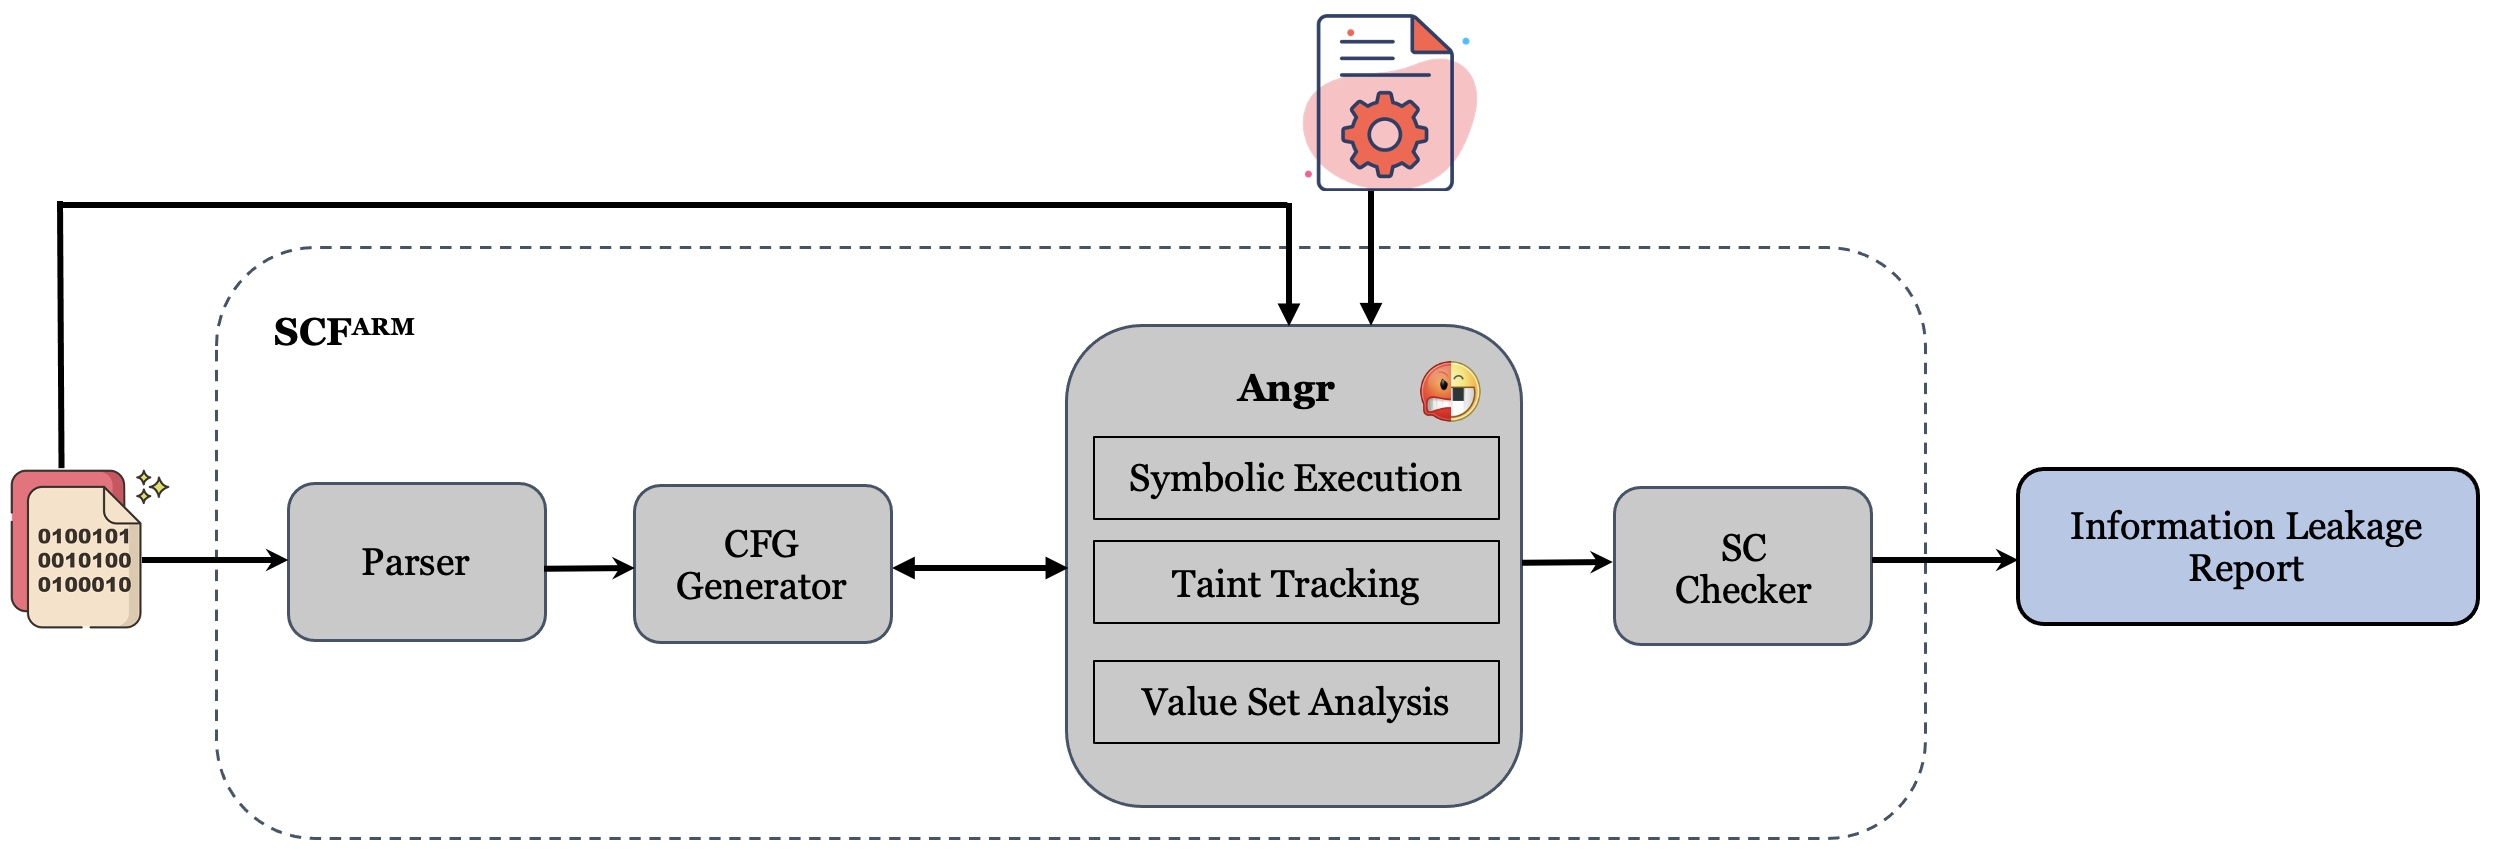
\includegraphics[width=.9\textwidth]{figures/SCFARM.jpg}
  \caption{Overview of \ac{SCF}\textsuperscript{ARM}}
  \label{fig:SCFARM}
\end{figure*}

We'll now provide a concise summary of each element and their practical implementations:

\textbf{Parser.} We employ this component to convert the input binary into assembly language. Initially, we utilize the pyelftools\footnote{https://github.com/eliben/pyelftools} Python library to locate the starting point of instructions within the binary. Subsequently, we leverage the Capstone\footnote{http://www.capstone-engine.org/} disassembler to translate the binary into ARMv8-M instructions, generating mnemonic codes and symbolic representations of processor instructions. This disassembly process allows us to extract essential details such as opcodes, addresses, and instruction lengths. Finally, we determine the required clock cycles for executing each instruction based on the specifications outlined in the ARMv8-M Architecture Reference Manual \cite{armv8m_ref_manual}.

\textbf{CFG Generator.} This component is responsible to construct an accurate program Control Flow Graph (CFG) using the NetworkX \cite{networkX} Python library. This component establishes a mutual connection with the subsequent component, enabling the retrieval of the target address for ‘branch and exchange’ instruction \textit{BX <Rm>} through \ac{VSA} in Angr. The resulting graph facilitates the identification of execution point predecessors and successors, aiding in computing control dependence regions for branches and inferring loops within assembly programs.

\textbf{Angr.} Utilizing a JSON-formatted configuration file that lists the starting function's arguments derived from high-level code to determine taint sources (i.e., highly sensitive inputs). This component employs Angr's annotation system to mark registers and memory cells containing confidential data with a taint label. It associates arguments with their corresponding registers following the ARMv8-M calling conventions \cite{armv8m_ref_manual}. These taint tags propagate during the symbolic execution of the input binary. Our taint analyzer tracks both explicit and implicit flows. Upon completion of symbolic execution, the component presents a list of tainted registers and memory cells for subsequent analysis. 

\textbf{SC Checker.} This module performs static analysis to identify potential side channel leaks within ARMv8-M assembly programs. Our \ac{SCF}\textsuperscript{ARM} tool currently detects vulnerabilities falling into four distinct classes:

\begin{itemize}

\item Timing Channel: Detected when a program exhibits different execution times depending on the secret input. \ac{SCF}\textsuperscript{ARM} detects these leaks by measuring the overall running times of if/else regions within the secret-dependent branches.

\item BUSted Vulnerability: Recognized when a program includes store/load instructions with different time offsets inside the if/else regions of a secret-dependent branch.

\item Nemesis Vulnerability: Identified when a program displays varying execution times for at least one instruction within the if/else regions of a secret-dependent branch.

\item Storage Channel: Flagged if there is an undesired information flow from secret inputs to observable output, such as return registers or non-secure memory.

\end{itemize}
